\section{Software architecture and design}
\label{chapter2}

\paragraph
{}
	%If the acc is turned on, a 5ms task on node2 periodically requests distance readings from node1. Out of the readings it derives the new speed of the car. In alarm situations, e.g. failed readings, an object gets too close, no bt communication available, ... the acc turns off and alarms the driver to take over.
When the ACC is activated, Node 2 executes a periodic task every 5 ms to request distance measurements from Node 1. Based on these readings, it calculates the updated speed of the virtual car. In case of an alarm situation - such as invalid or missing sensor data, an object detected at critical distance, or a loss of Bluetooth communication - the ACC is automatically deactivated and the driver is alerted to take control.

\subsection{Software modules}

\begin{itemize}
	\item bt\_connection on node1 and node2
	\item acc\_control on node2
	\item proximity\_reader on node1
	\item display\_control on node2
	\item fault\_injection\_agent
\end{itemize}


\subsubsection{Safety related modules}
	% \begin{enumerate}
	% 	\item Modul x: \\
	% 		Description:\\
	% 		Functions:\\
	% 		Data:\\
	% 		Requirements see: \ref{req.1.1}, .... \\
	% \end{enumerate}


\subsubsection{Security related modules}

\subsubsection{Modules with no influence on Safety and Security}

\subsection{Libraries}

Description of used function with parameters.


\subsection{Interrupts}

Definition of priorities.

\subsection{Pinout}

\subsection{GUI}

\ref{fig:gui} shows the dashboard GUI, containing the controls for accelerating and decelerating the vehicle, and for activating adaptive cruise control. It also contains elements showing the vehicles current speed, the distance to the nearest object in front of the car, and the status of the ACC system.

\begin{figure}[h]
	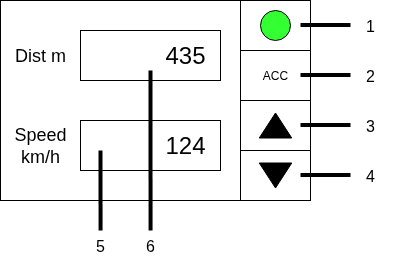
\includegraphics[height=50mm]{images/GUI.png}
	\centering
	\caption{Dashboard GUI}
	\label{fig:gui}
\end{figure}

\begin{enumerate}
  \item ACC Status LED: Shows the status of the ACC system, green if it is in an operational state, red, if ACC  is in a failed state.
  \item ACC Button: Push Button to activate ACC. Can only be pushed if ACC is in operational state and not turned on already.
  \item Accelerate Button: Increases the vehicle speed by 5 km/h (up to 200 km/h), deactivates ACC, if it was active.
  \item Decelerate Button: Decreases the vehicle speed by 5 km/h (down to 0 km/h), deactivates ACC, if it was active.
  \item Speed Display: Shows current vehicle speed
  \item Distance Display: Shows distance of the nearest object in front of the vehicle, does not display anything if ACC is in failed state.
\end{enumerate}
